\documentclass[a4paper, 11pt]{article}
\usepackage[total={6in, 8in}, margin=1.2in, bottom=1in]{geometry}
\usepackage{bera}
\usepackage{color}
\usepackage{graphicx}
\usepackage{caption}
\usepackage{enumitem}
\usepackage{bigints}
\usepackage{relsize}
\usepackage{amsmath}
\usepackage{multirow}
\usepackage{fixltx2e}
\usepackage{adjustbox}
\usepackage[utf8]{inputenc}
\usepackage{epigraph}
\usepackage{floatrow}
\usepackage{subcaption}
\usepackage{mwe}
\usepackage{float}
\usepackage{listings}
\usepackage{csquotes}
\usepackage{xcolor}
\usepackage{tabto}
\usepackage[linesnumbered,algoruled,boxed,commentsnumbered]{algorithm2e}
\usepackage{qtree}
\title{ \huge \textbf{ Software Systems Lab: OutLab 5}\\
\huge \textbf{\LaTeX (80 marks)}}
\author{\Large \text{Code Warriors}\\
\normalsize 180050013\\
\normalsize 180050085\\
\normalsize 180050097\\
}
\date{12 September, 2019 }
\begin{document}
\maketitle


%\begin{titlepage}
%   \begin{center}
%       \vspace*{4cm}
% 
%       \huge \textbf{ Software Systems Lab: OutLab 5}
% 
%       \vspace{0.5cm}
%        \huge \textbf{\LaTeX (80 marks)}
% 
%       \vspace{1.2cm}
% 
%       \Large \text{Code Warriors}
% 
%       \vspace{0.5cm}
%      \normalsize 180050013
%     
%      \normalsize 180050085
%
%      \normalsize 180050097 
%      
%      \vspace{1cm}
%      
%      \large 12 September, 2019
%      
%   \end{center}
%\end{titlepage}

\newpage

\tableofcontents
\pagenumbering{arabic}
\newpage

This is a \LaTeX document for the course \textbf{Software Systems Lab} with course code \textsl{CS 251}. You need to replicate the document. Spacing need not be matched perfectly but page numbers should be. \textbf{1 mark is for the title page.}. Bonus marks will be given only if you score full (80/80) in the rest.
\section{Introduction (4 marks)}
\quad \tab
\textbf{\LaTeX} is a word processor and document markup language. It is distinguished
from typical word processors such as Microsoft Word and Apple Pages in that
the writer uses plain text as opposed to formatted text, relying on markup
tagging conventions to define the general structure of a document (such as
article, book, and letter), to stylise text throughout a document (such as \textbf{bold}
and \textit{italic}), and to add citations and cross-referencing. A \textbf{\TeX} distribution such
as \textbf{\TeX  Live} or \textbf{MikTeX} is used to produce an output file (such as PDF or DVI)
suitable for printing or digital distribution.
\bigbreak
\textbf{\LaTeX} is used for the communication and publication of scientific documents
in many fields, including mathematics, physics, computer science, statistics,
economics, and political science. It also has a prominent role in the preparation
and publication of books and articles that contain complex multilingual materi-
als, such as Sanskrit and Arabic. \textbf{\LaTeX} uses the TeX typesetting program for
formatting its output, and is itself written in the TeX macro language.
\bigbreak
\textbf{\LaTeX} is widely used in academia. \textbf{\LaTeX} can be used as a standalone docu-
ment preparation system, or as an intermediate format. In the latter role, for
example, it is often used as part of a pipeline for translating DocBook and other
XML-based formats to PDF. The typesetting system offers programmable desk-
top publishing features and extensive facilities for automating most aspects of
typesetting and desktop publishing, including numbering and cross-referencing
of tables and figures, chapter and section headings, the inclusion of graphics,
page layout, indexing and bibliographies.
\bigbreak
Below are some of the basic packages which you’ll be using. For other
required packages, search over the net :).

\subsection{graphicx package}
This package is used to import tables, and figure in the document. Our
document type is article, and we are currently using a4 type paper with the
following margin geometry: (total={6in, 8in}, margin=1.2in, bottom=1in),
which is specified in the beginning.

\subsection{amssymb package}
This package is used to import mathematical symbols in the document. We encapsulate the mathematical equations and symbols under \$, and they are changed to maths symbols.

\section{Pointers (3 + 2 + 1 marks)}
Here we are using \textbf{itemize} to generate unordered list.
\begin{itemize}
\setlength\itemsep{2em}
	\item \LaTeX typesets a file of text using the TEX program.
	\item \LaTeX is widely used in academia for the communication and publication of scientific documents in many fields, including mathematics, physics, computer science, statistics, economics and political science.
	\item \LaTeX can be used as a standalone document preparation system or as an intermediate format.
	\item \textbf{We have used renewcommand for the bullets to be bigger.}
	\item Look at the \textbf{item separation space}, and \textbf{change it} accordingly.
\end{itemize}
For ordered lists we use \textbf{enumerate}.

\begin{enumerate}[label=\Roman*.]
\setlength\itemsep{1em}
	\item \LaTeX typesets a file of text using the TEX program.
	\item \LaTeX is widely used in academia for the communication and publication of scientific documents in many fields, including mathematics, physics, computer science, statistics, economics and political science.
	\item \LaTeX can be used as a standalone document preparation system or as an intermediate format.
	\item \LaTeX is intended to provide a high-level language that accesses the power of TeX in an easier way for writers.
\end{enumerate}
\begin{enumerate}[label=(\alph*)]
	\item \LaTeX typesets a file of text using the TEX program.
	\item \LaTeX is widely used in academia for the communication and publication of scientific documents in many fields, including mathematics, physics, computer science, statistics, economics and political science.
\end{enumerate}

Following is another type of a pointer (\textbf{description}).

\begin{description}
	\item[\textbf{CS 213}] Data structures and Algorithm
	\item[\textbf{CS 215}] Data Analysis and Interpretation
	\item[\textbf{CS 251}] Software Systems Lab
\end{description}

\section{Mathematical formulae and notations (15 marks)}
\subsection{Equation Array (4 marks)}
\begin{eqnarray}
	\cos^3{\theta} + \sin^3{\theta} & = & (\cos{\theta} + \sin{\theta})(\cos{2\theta} - \cos{\theta}\sin{\theta})\\
	& = & (\cos{\theta} + \sin{\theta})(1 - \cos{\theta}\sin{\theta})\\
	& = & (\cos{\theta} + \sin{\theta})(1/2)(2 - 2\cos{\theta}\sin{\theta})(3)\\
	& = & (1/2)(\cos{\theta} + \sin{\theta})(2 - \sin(2\theta))
\end{eqnarray}

\subsection{Prepositional Formulae using Various Operators (2 marks)}

$ (\exists x)(\phi(x) \wedge \psi(x)) \leftrightarrow ((\exists x)\phi(x) \wedge (\exists x)\psi(x)) $
\\ \\
$ (\exists x)(\phi(x) \wedge \psi(x)) \to ((\exists x)\phi(x) \wedge (\exists x)\phi(x) \wedge (\exists x)\psi(x)) $

\subsection{Alphabets (3 marks + 1 mark for table)}
\vspace{0.5cm}
\begin{center}
\renewcommand{\arraystretch}{1.7}
\begin{tabular}{|c|c|}
\hline

	Binary Operators: & $ \times \otimes \oplus \cup \cap $  \\
	\hline

	Relation Operators: & $ \subset \supset \subseteq \supseteq < >$ 	\rule{0pt}{4ex} \\
	\hline
	Others: & $ \int \oint \sum \prod $ 	\rule{0pt}{4ex} \\
	\hline
\end{tabular}
\end{center}

\subsection{Mathematical Formulas (5 marks) }
\begin{enumerate}
	\item $\mathlarger{ \int_{a}^{b} x^3 dx = \frac{1}{4}x^4\bigg|_{a}^b }$
	\item $\mathlarger{ \frac{\pi}{4} = 4\sum_{n=0}^{\infty}\frac{(-1)^n}{(2n+1)5^{2n+1} } - \sum_{n=0}^{\infty} \frac{(-1)^n}{(2n+1)239^{2n+1}} }$ 
	\item $\mathlarger{ \pi =\frac{3\sqrt{3}}{4} - 24\sum_{n=0}^{\infty} \frac{\frac{(2n)!}{(n)}}{2n+1(2n+1)4^{2n+1} }}$
	\item $\mathlarger{\frac{1}{\pi} = \frac{2\sqrt{2}}{9801} \sum_{n=0}^{\infty} \frac{(4n)!(1103+26390n)}{(n)!^4396^{4n}}}$
	\item $\mathlarger{ \sum_{i=0}^{\left[\frac{n}{2}\right[} {{x_{i,i+1}^{i^2}}\choose{\left[\frac{i+3}{3}\right[}} \frac{\sqrt{\mu (i)^{\frac{3}{2}} (i^2-1)}}{\sqrt[3]{\rho(i)-2} + \sqrt[3]{\rho(i) -1}} }$
\end{enumerate}

\newpage
\section{Tables (10 marks) }
To combine rows a package must be imported with in your preamble, then you
can use the XXXXXXX command in your document. The table below includes
mathematical notations, which you can produce by embedding the expression
in \$ \$ delimiters. For subscript, use underscore and for superscript, use carrot.

\renewcommand{\arraystretch}{1}

\begin{table}[h!]
\begin{adjustbox}{max width=\textwidth}
%\centering
\begin{tabular}{|cc|c|c|c|c|c|c|c|c|c|c|}
	\cline{4-12}
	\multicolumn{3}{c|}{\multirow{2}{*}{}} & \multicolumn{5}{c}{\textbf{Basic Properties}} & \multicolumn{4}{|c|}{\textbf{Readability}} \\
	\cline{4-12}
	\multicolumn{3}{c|}{} & \textbf{WC} & \textbf{SC} & \textbf{C-W} & \textbf{S-W} & \textbf{W-S} & \textbf{FK} & \textbf{GF} & \textbf{SMOG} & \textbf{LEX} \\
	\hline
	\multicolumn{2}{|c|}{\multirow{2}{*}{\textit{Baseline}}} & Mean & 0.84 & 0.41 & \textbf{0.56} & \textbf{0.46} & \textbf{0.55} & \textbf{0.60} & 0.56 & 0.57 & 0.63 \\
	\cline{3-12}
	\multicolumn{2}{|c|}{} & SD & 0.07 & 0.08 & 0.06 & 0.07 & 0.05 & 0.05 & 0.06 & 0.07 & 0.05 \\
	\hline
	\hline
	\multicolumn{2}{|c|}{\multirow{2}{*}{\textit{ScaComph}}} & Mean & 0.89 & 0.46 & 0.53 & 0.43 & 0.53 & 0.58 & 0.54 & 0.56 & 0.62 \\
	\cline{3-12}
	\multicolumn{2}{|c|}{} & SD & 0.05 & 0.08 & 0.05 & 0.06 & 0.06 & 0.05 & 0.05 & 0.06 & 0.05 \\
	\hline
	\hline
	\multicolumn{2}{|c|}{\multirow{2}{*}{\textit{ScaComph}}} & Mean & \textbf{0.92} & \textbf{0.48} & 0.55 & 0.45 & 0.53 & 0.59 & \textbf{0.58} & \textbf{0.61} & \textbf{0.64} \\
	\cline{3-12}
	\multicolumn{2}{|c|}{} & SD & 0.04 & 0.07 & 0.05 & 0.04 & 0.05 & 0.04 & 0.04 & 0.04 & 0.04 \\
	\hline
	
\end{tabular}
\end{adjustbox}
%\end{center}

\caption {Table depicting the use of both multirow and multicolumn}


\end{table}

{\Large In table 1 above, we try to demonstrate all the fea-
tures required to be demonstrated in a table. We use
multiple newline, we use a package to enable the use
of multiple rows, and multiple columns in the table.
Additionally, We have also drawn lines from specific
column to column. We also use box resizing with a
width specifier for resizing the box within the limits of
the document, and avoid any overflow.}

\newpage
\section{Image Insert (7 + 7 marks)}
\begin{center}
Now, we will import images side by side in the same document.
\end{center}

\begin{figure}[H]
\begin{floatrow}
	\ffigbox{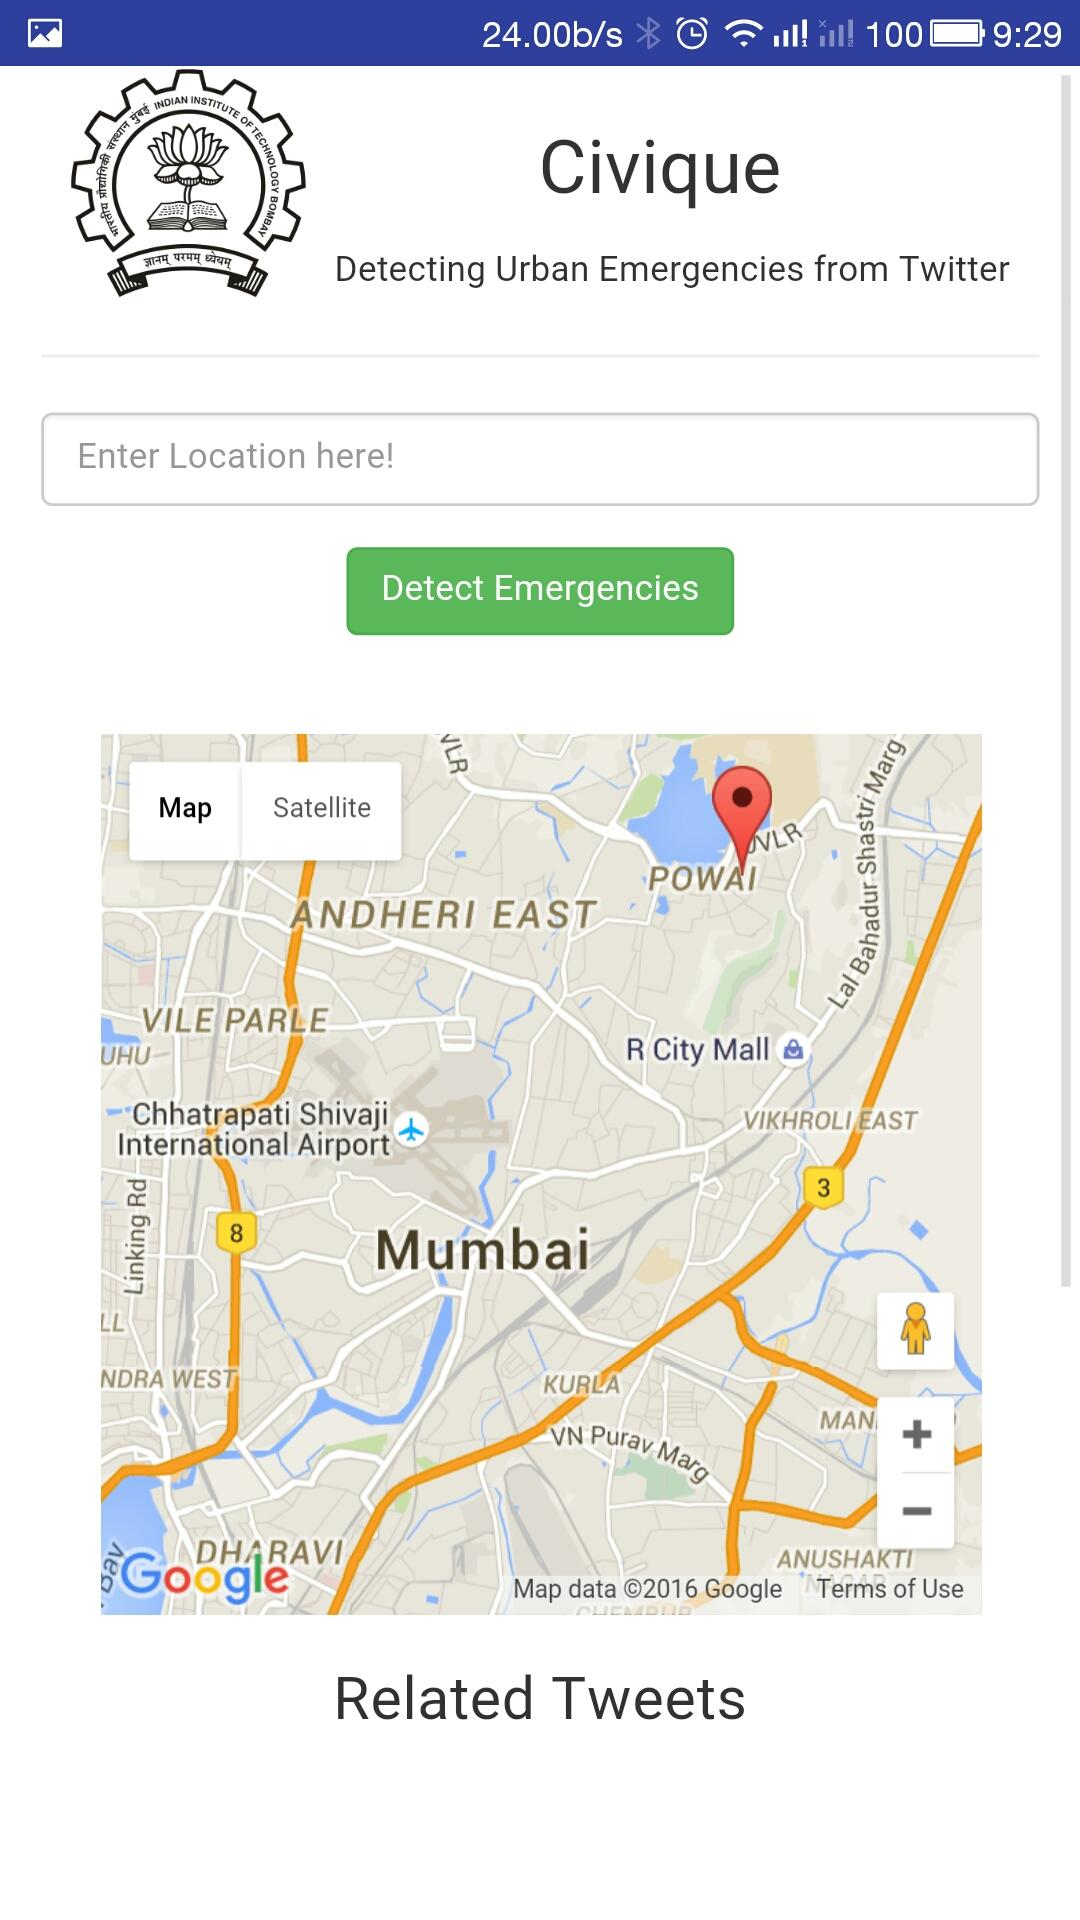
\includegraphics[scale = 0.14]{1.jpg}}{\caption{Screenshot: Mobile Interface}\label{figa}}
	\hspace{-0.4cm}
	\ffigbox{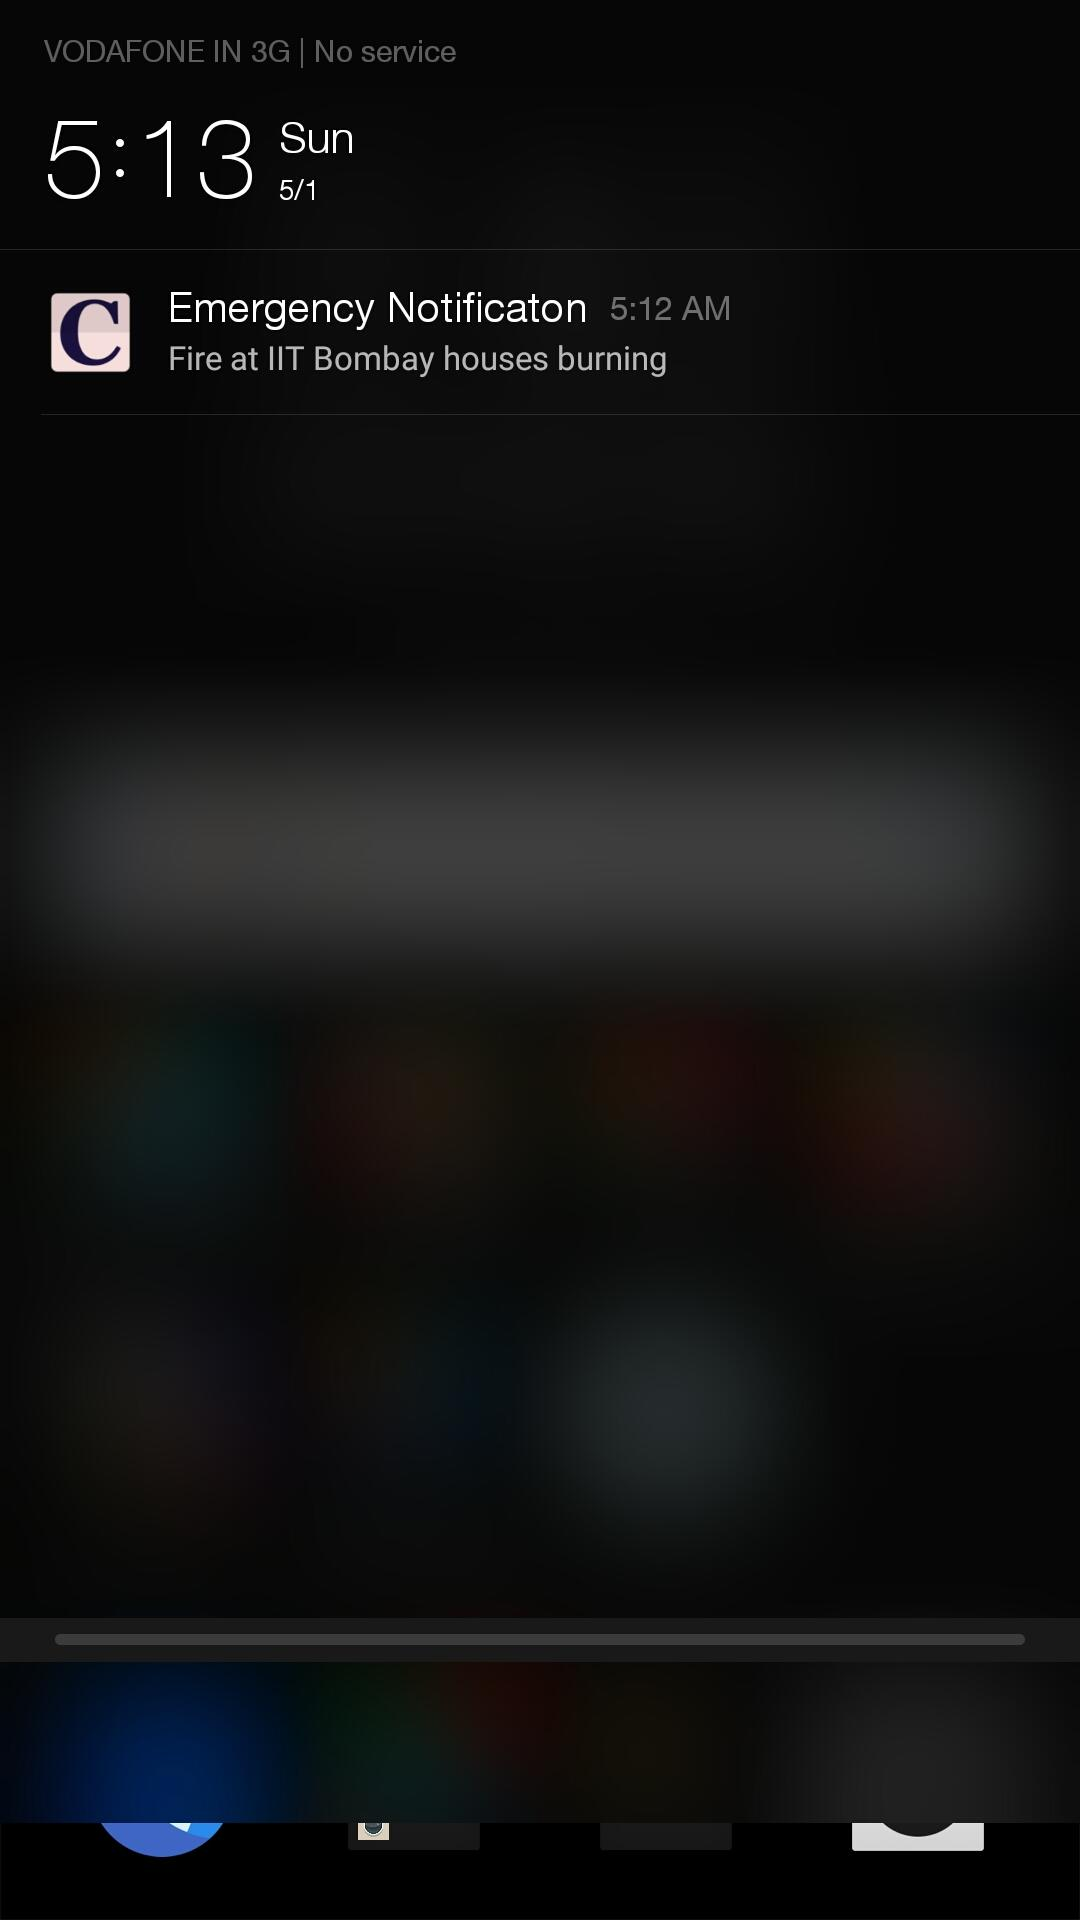
\includegraphics[scale = 0.14]{2.jpg}}{\caption{Screenshot: Generated Notification}\label{figb}}
\end{floatrow}
\end{figure}

The images have been put in, and they are side by side in the same document on the same page. We have used the package \textbf{floatrow} and \textbf{graphicx} to import images on Page 6.

In case you would like to see an alternative method to align the images, for instance images as \textbf{subfigures}, here it is.

\begin{figure}[H]
%\centering
\begin{subfigure}{.5\textwidth}
  \centering
  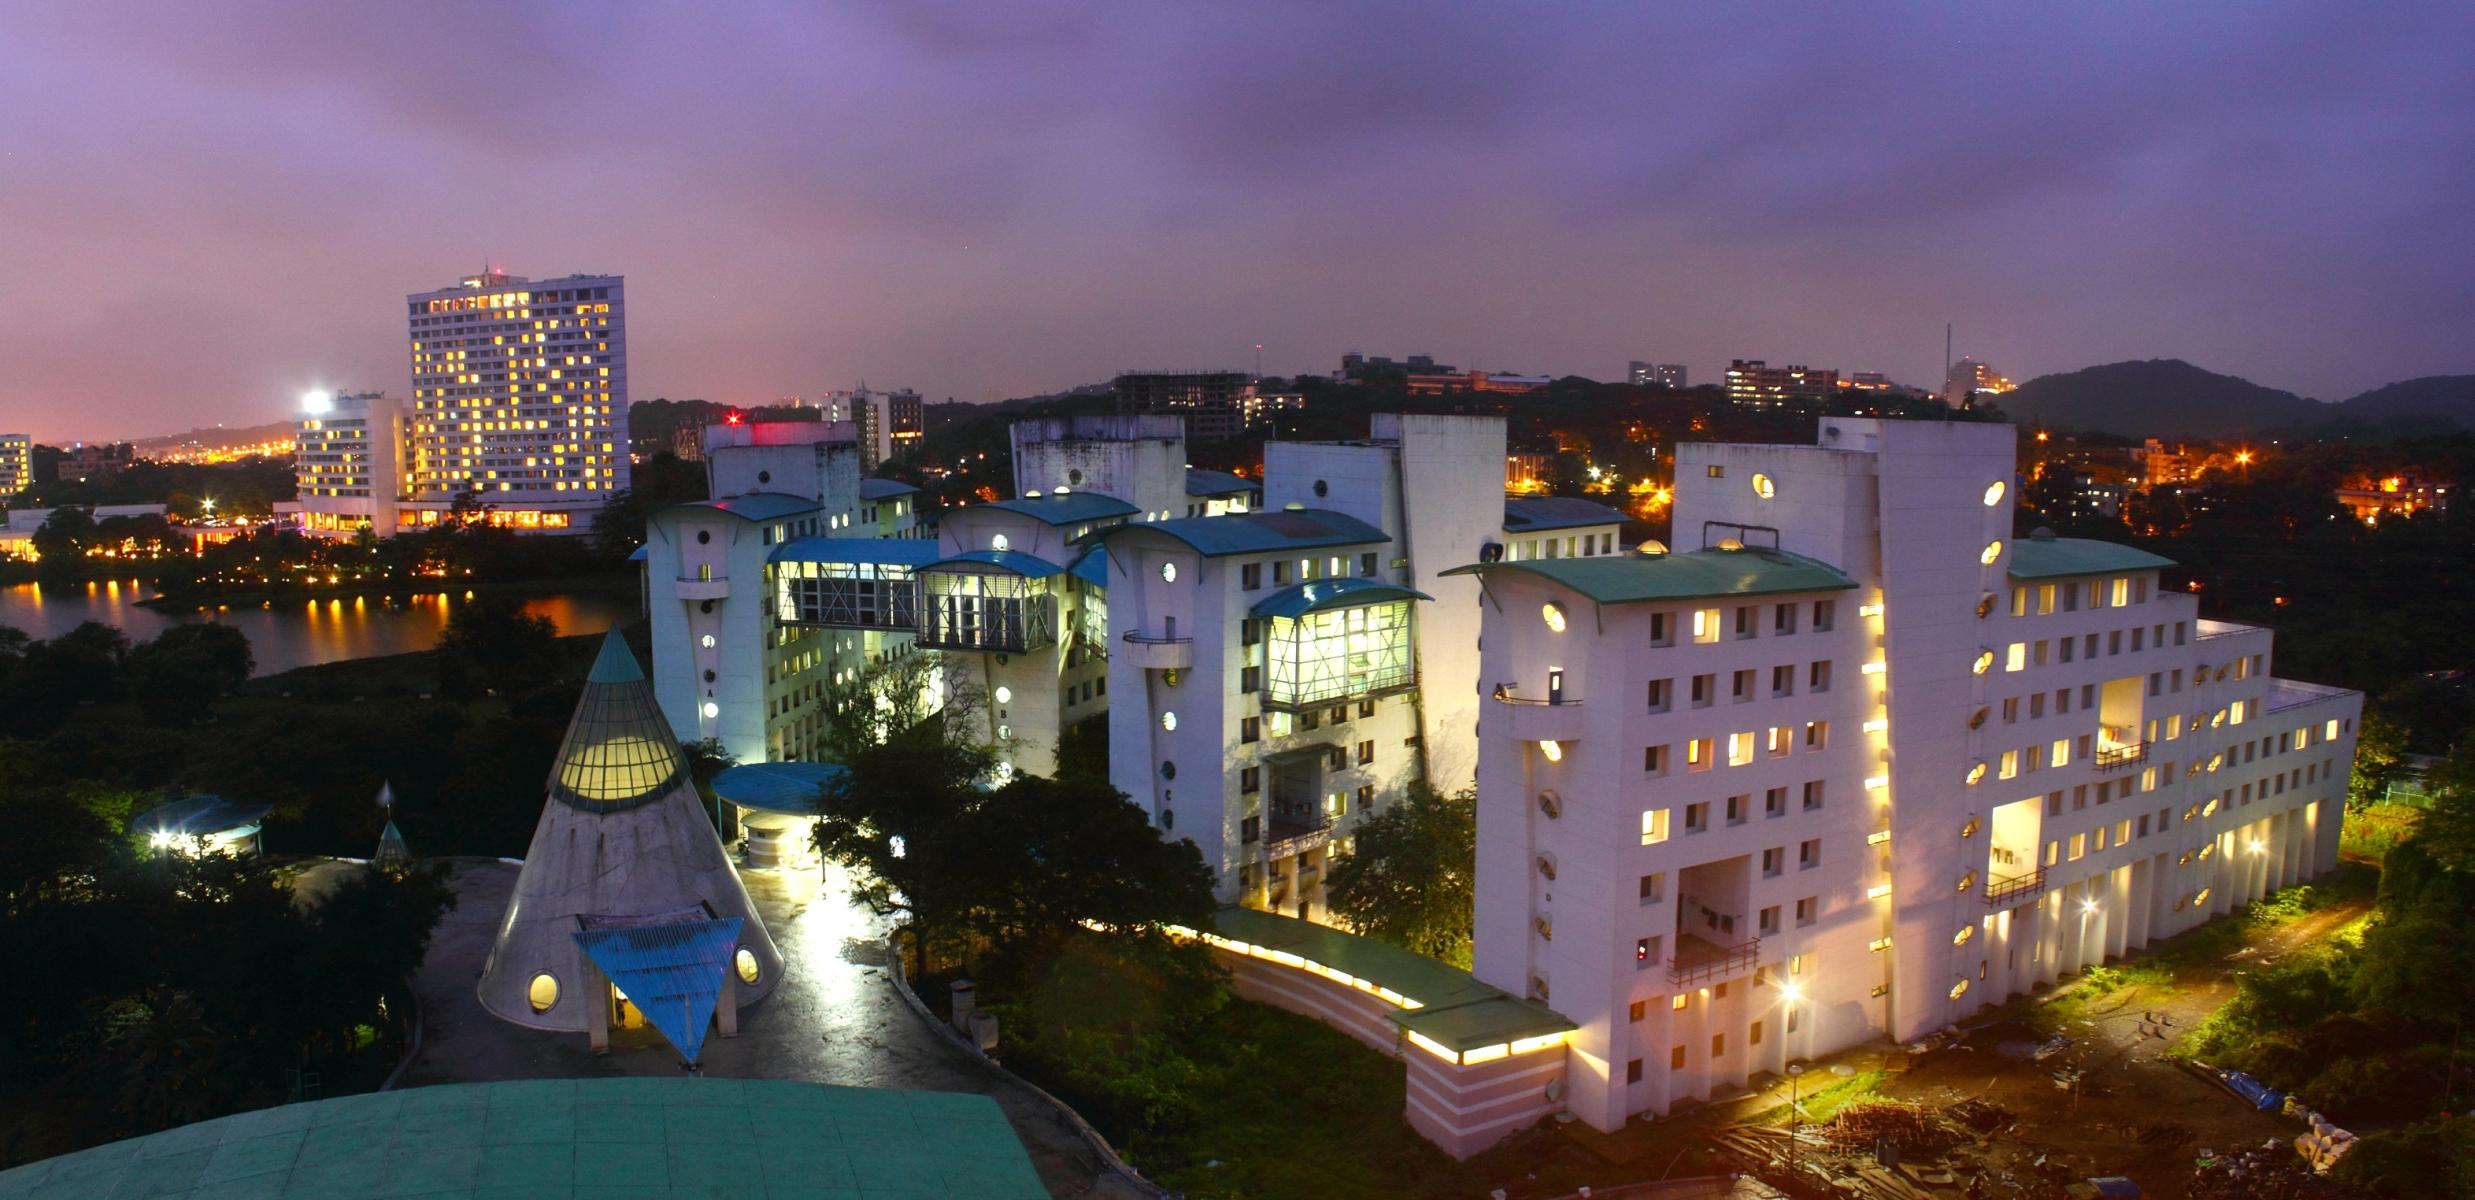
\includegraphics[width=.85\linewidth, height=3.5cm]{3.jpg}
  \caption{Caption 1}
  \label{fig:sub1}
\end{subfigure}%
\begin{subfigure}{.5\textwidth}
  \centering
  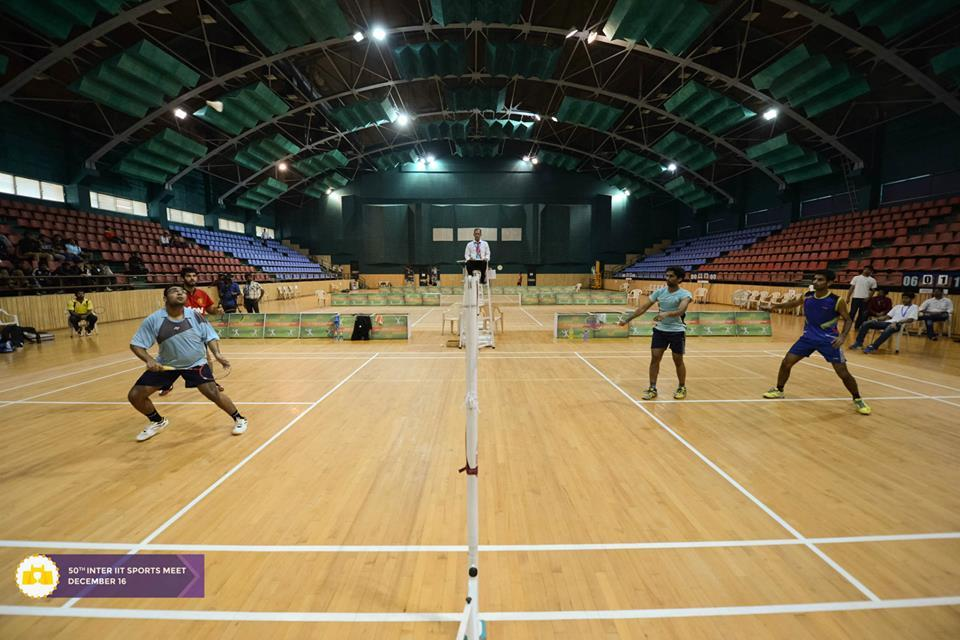
\includegraphics[width=.85\linewidth]{4.jpg}
  \caption{Caption 2}
  \label{fig:sub2}
\end{subfigure}
\caption{Caption for this figure with two images}
\label{fig:test}
\end{figure}

\newpage
\section{Quotation an Citation (4 marks)}

\subsection{Quotation (2 marks)}
The margins of the quotation environment are indented on both the left and the
right. The text is justified at both margins. Leaving a blank line between text
produces a new paragraph. The package \textbf{csquotes} offers a multilingual solu-
tion to quotations, with integration to citation mechanisms offered by BibTeX.
This package allows one for example to switch languages and quotation styles
according to babel language selections.

\begin{quote}
"Unlike the quote environment, each paragraph is indented nor- mally.
It’s important to remark that even if you are typing quotes on English
there are different quotation marks used in English (UK) and English
(US)."
\end{quote}

\subsection{Citation (2 marks)}
Latex \cite{first} is a document preparation system for typesetting program. It is used
to create different types of document structures. A Latex file (.tex) is created
using any text editor (vim, emacs, gedit, etc.). There are also many LaTeX
IDEs like Kile, TexStudio, etc.. The Latex code is then compiled which creates
a standard (.pdf) file. Thus, the presentation of the document does not change
on different machines.
\\
Type style\cite{second} is used to indicate logical structure. Emphasized text appears in
italic style type and input in typewriter style. Type style is specified by three
components: shape, series, and family.\\

There are two ways of producing a bibliography\cite{third}. You can either produce
a bibliography by manually listing the entries of the bibliography or producing
it automatically using the BibTeX program of LaTeX. The bibliography style can
be declared with bibliographystyle command, which may be issued anywhere
after the preamble. The style is a file with .bst extension that determines how
bibliography entries will appear at the output, such as if they are sorted or not,
or how they are labeled etc. The extension .bib is not written explicitly. There
are many standard bibliography style files. Two of them that are compatible
with IIT thesis manual are plain.bst and alpha.bst. They are part of the LaTeX
package; a student does not need to download it. The plain.bst and alpha.bst
styles are explained below. The symbols in a math formula fall into different
classes that correspond more or less to the part of speech each symbol would
have if the formula were ex pressed in words. Certain spacing and position-
ing cues are traditionally used for the different symbol classes to increase the
readability of formulas. \cite{fourth}

My citations are in proper order as per references ref1, ref2, ref3, and ref4.
\newpage
\section{Algorithm and Pseudo Code (22 marks)}
\subsection{Listing (10 marks)}
\rule{\textwidth}{0.1pt}
\definecolor{codegreen}{rgb}{0,0.6,0}
\definecolor{codegray}{rgb}{0.5,0.5,0.5}
\definecolor{codepurple}{rgb}{0.58,0,0.82}
\definecolor{backcolour}{rgb}{1,1,1}

\lstdefinestyle{mystyle}{
    backgroundcolor=\color{backcolour},   
    commentstyle=\color{codegreen},
    keywordstyle=\color{blue},
    numberstyle=\tiny\color{backcolour},
    stringstyle=\color{codepurple},
    basicstyle=\large,
    breakatwhitespace=false,         
    breaklines=true,                 
    captionpos=b,                    
    keepspaces=true,                 
    numbers=left,                    
    numbersep=5pt,                  
    showspaces=false,                
    showstringspaces=false,
    showtabs=false,                  
    tabsize=2
}
\lstset{style=mystyle}

\begin{lstlisting}[language=C++]
//Breadth First Search Function
void BFS(list<long long int> queue,long long int length
	){
	long long int v ;
	if (queue.empty())
		return ;
	list<long long int>::iterator i;
	list<long long int> queue_temp;
	while(!queue.empty()){
		v=queue.front() ;
		queue.pop_front();
		for(i=adj[v].begin();i!=adj[v].end();i++){
			if(!pro_ver[*i]){
				result[*i]=length;
				queue_temp.push_back(*i);
				pro_ver[*i]=true;
				adj[*i].remove(v);
				}
			}
		}
	BFS(queue_temp , length+1);
}
\end{lstlisting}
\newpage

\subsection{Algorithmic (12 marks)}
\RestyleAlgo{boxruled}
\begin{algorithm}[H]
\caption{How to write algorithms}
\SetAlgoLined
\SetKwInput{KwData}{Input}
\KwData{A graph Graph and a starting vertex root of Graph}
\SetKwInput{KwResult}{Output}
\KwResult{All vertices’s reachable from root labeled as explored.}
Breadth-First-Search(Graph, root):

\For{each node n in Graph  :}{
$n$.\textbf{distance} = INFINITY

$n$.\textbf{parent} = NIL
}
create empty \textbf{queue} Q

root.\textbf{distance} = 0

Q.\textbf{enqueue}(root)

\While{Q is not empty :}{
current = Q.dequeue()

\For{each node n that is adj acent to current}{
\If{n.\textbf{distance} == INFINITY}{
n.\textbf{distance} = current.\textbf{distance} + 1 n.\textbf{parent} = current

Q.\textbf{enqueue}(n)
}
}
}
\end{algorithm}
\section{Tree (Bonus - 4 marks)}
\Tree [.If-statement if exp then [.S [.if if else then S ] ] ]

\newpage
\section{Exotic Features (Bonus - 6 marks)}

\subsection{Epigraph Style (3 marks)}

\subsection*{Chapter 1: Theory of Life}
 
\epigraph{"failure will never overtake me
if my determination to succeed
is strong enough."}{\textit{og mandino}}

\subsection{Minipage (3 marks)}

%\begin{figure}[h]

\fbox{
\begin{minipage}[t]{0.45\textwidth}
\textsl{{\LaTeX} typesets a file of text using the
TEX program and the {\LaTeX} “macro
package” for TEX. That is, it processes
an input file containing the text of a
document with interspersed commands
that describe how the text should be
formatted. {\LaTeX} files are plain text
that can be written in any reasonable
editor. In the {\LaTeX} input file, a com-
mand name starts with a followed by
either (a) a string of letters or (b) a sin-
gle non-letter. Arguments contained in
square brackets, [ ], are optional while
arguments contained in braces, \{\}, are
required. {\LaTeX} is case sensitive. En-
ter all commands in lower case unless
explicitly directed to do otherwise.}
\end{minipage}}

%\end{figure}

\newpage
\section{Bibliography (4 marks)}
4 marks for references using .bib file, otherwise 2 marks.

\begin{thebibliography}{9}
\bibitem{first}
Firuza Aibara. LaTeX - Fundamental Research Group - IIT Bombay.
http://www.it.iitb.ac.in/frg/wiki/index.php/LaTeX/, 2016.

\bibitem{second}
Leslie Lamport. Latex. \textsl{Addison-Wesley}, 1994.

\bibitem{third} 
Helmut Kopka and Patrick W Daly. \textsl{A guide to latex}. 1995.

\bibitem{fourth}
Michael Downes. Short math guide for latex. \textsl{American Mathematical Society}, 2002.

\end{thebibliography}
 

\end{document}
